\documentclass[table]{beamer}

% Customize slide appearance
\mode<presentation>
{
  \usetheme{Warsaw}
  \setbeamercovered{transparent}
}

\usepackage[english]{babel}
\usepackage{times}
\usefonttheme[onlymath]{serif} 
\setbeamertemplate{navigation symbols}{}

% You can add any graphics to every slide by following command:
% \logo{\resizebox{0.1\textwidth}{!}{\includegraphics{col_small}}}
% \logo{\resizebox{0.2\textwidth}{!}{\includegraphics{imperialblue}}}

% Uncomment this, if you want the table of contents before each subsection.
% However, to edit slides in TeXWord avoiding this feature is good idea.
% \AtBeginSubsection[]
% {
%   \begin{frame}<beamer>
%     \frametitle{Outline}
%     \tableofcontents[currentsection,currentsubsection]
%   \end{frame}
% }

% If you wish to uncover everything in a step-wise fashion, uncomment
% the following command: 
%\beamerdefaultoverlayspecification{<+->}
\xdefinecolor{keyword}{rgb}{0,0,1}
\xdefinecolor{ctext}{rgb}{0.64,0.08,0.08}
\xdefinecolor{cline}{rgb}{0.17,0.57,0.69}
\xdefinecolor{comment}{rgb}{0,0.5,0.0}
\newif\ifschigh\schighfalse
\newcommand{\kw}[1]{\ifschigh\textcolor{red}{#1}\else\textcolor{keyword}{#1}\fi}
\newcommand{\kt}[1]{\ifschigh\textcolor{red}{#1}\else\textcolor{ctext}{#1}\fi}
\newcommand{\kc}[1]{\ifschigh\textcolor{red}{#1}\else\textcolor{comment}{#1}\fi}
\addtobeamertemplate{alerted text begin}{\global\schightrue%
}{}
\defbeamertemplate*{alerted text end}{default}{\global\schighfalse%
}

\newcounter{sckll}
\newcommand{\kr}{\setcounter{sckll}{1}}
\newcommand{\krr}[1]{\setcounter{sckll}{#1}}
\newcommand{\klvalue}{\ifnum\value{sckll}<10{\hphantom{0}}\fi\arabic{sckll}\addtocounter{sckll}{1}}
%\newcommand{\kl}{\ifschigh\textcolor{red}{\klvalue}\else\textcolor{cline}{\klvalue}\fi\hspace{2ex}}
\newcommand{\kl}{}

\newcounter{scpl}
\newcommand{\kp}{\arabic{scpl}\addtocounter{scpl}{2}}
\newcommand{\kpr}{\setcounter{scpl}{3}}

\let\oldurl=\url
\renewcommand{\url}[1]{\textcolor{blue}{\oldurl{#1}}}

\usepackage{tikz, pgfbaseplot, pgflibrarysnakes,pgflibraryarrows}

\begin{document}

% Title Data. We keep it after \begin{document} 
% to enable editing text in BaKoMa TeX Word.

\title[C for Science - Lecture 5]{Computing in C for Science}
\subtitle{Lecture 5 of 5}

% Use the \inst command to identify several affiliations.
\author[Steven Capper]{Dr. Steven Capper \\ {\tt steven.capper99@imperial.ac.uk}\\
\url{http://www2.imperial.ac.uk/~sdc99/ccourse/}}

\date{$14^\text{th}$ December 2011}

\subject{C for Science} % Should be passed to PDF [YNI]
{
\logo{\includegraphics[width=0.30\textwidth]{imperialblue}}
\begin{frame}
  \titlepage
\end{frame}
}

\begin{frame}[fragile]
\frametitle{Cryptic C - What do I do?}
\begin{semiverbatim}
\scriptsize
\kr\kl\kw{void} whatdoIdo(\kw{double} *A, \kw{double} * B, \kw{double} *C,
\kl                    \kw{unsigned int} L, \kw{unsigned int} M,
\kl                    \kw{unsigned int} N)
\kl\{
\kl   \kw{unsigned int} i, k;
\kl   \kw{double} temp, *bptr, *bend, *cptr;
\kl
\kl   \kw{for}(i=0; i < L; i++)
\kl   \{
\kl      \kw{for} (k=0; k < M; k++)
\kl      \{
\kl         temp = A[i*M+k];
\kl         cptr = &C[i*N];
\kl         bptr = &B[k*N];
\kl         bend = &B[(k+1)*N];
\kl         \kw{while} (bptr < bend)
\kl            *cptr++ += temp*(*bptr++);
\kl      \}
\kl   \}
\kl\}
\end{semiverbatim}
\end{frame}

\begin{frame}
\frametitle{Projects and Makefiles}
\begin{itemize}
\item It is possible (and encouraged) to build a program from multiple {\tt .c} files.
\item This maximises the portability of the code, and
\item Speeds up compiling - if we only change one {\tt .c} file we only need to recompile one file...
\item Visual Studio manages programs in to so-called \emph{projects}, and everything is done graphically.
\item UNIX systems have a very powerful program called {\tt make} which manages projects. Information for building programs is stored in a {\tt Makefile}.
\end{itemize}
\end{frame}

\begin{frame}[fragile]
\frametitle{A sample {\tt Makefile}}
\framesubtitle{There are many ways of writing one, this is mine!}
\begin{exampleblock}{}
\begin{semiverbatim}
\scriptsize
CFLAGS = -O2 -DNDEBUG -Wall -ansi
LFLAGS = -lm
CC = gcc
CLEANFILES = crypticc.o matrixfunctions.o cryptic cryptic.exe

cryptic: crypticc.o matrixfunctions.o
         $(CC) crypticc.o matrixfunctions.o $(LFLAGS) -o cryptic
         
clean:
        touch $(CLEANFILES)
        rm $(CLEANFILES)
\end{semiverbatim}
\end{exampleblock}
\begin{itemize}
\item This compiles {\tt crypticc.c} and {\tt matrixfunctions.c}.
\item It then links them to produce {\tt cryptic.exe} (Cygwin) or {\tt cryptic} (UNIX).
\item It has two rules {\tt cryptic} (default) to build the program and {\tt clean} to clean up all the compiled output.
\end{itemize}
\end{frame}

\begin{frame}
\frametitle{Bytes (or {\tt char}s)}
\begin{itemize}
\item We've mentioned {\tt \kw{char}}s briefly so far, and used them extensively whilst drawing little attention to them.
\item {\tt \kw{char}} is the smallest data type in C, {\tt \kw{sizeof}(\kw{char})=1} byte (this is explicitly stated in the standard).
\item We can perform integer computations using {\tt \kw{char}} and {\tt \kw{unsigned char}}.
\item The most common use for {\tt \kw{char}} is as part of a string.
\item We can assign single letters as follows:
\begin{center}
{\tt \kw{char} letter = \kt{'a'};}
\end{center}
where we use single quotes.
\item An array of {\tt \kw{char}}s is specified using double quotes:
\begin{center}
\tt \kw{char} * name = \kt{"Steven"};
\end{center}
\end{itemize}
\end{frame}

\begin{frame}[fragile]
\frametitle{Demo of {\tt char}}
\begin{semiverbatim}
\scriptsize
\kr\kl\kw{\#include} \kt{<stdio.h>}
\kl
\kl\kw{int} main()
\kl\{
\kl   \kw{char} * name = \kt{"David"};
\kl   printf(name); \kc{/* not recommended, but allowed*/}
\kl   printf(\kt{"\\nname    = \%s\\n"}, name);
\kl   printf(\kt{"name[0] = \%c = \%d\\n}", name[0], name[0]);
\kl   \kw{return} 0;
\kl\}
\end{semiverbatim}
Gives the following output:
\begin{semiverbatim}
David
name    = David
name[0] = D = 68
\end{semiverbatim}
\end{frame}

\begin{frame}
\frametitle{Layout of a String in Memory}
Given: {\tt \kw{char} * string = \kt{"A string in C!"};}
In memory this looks like:
\begin{center}
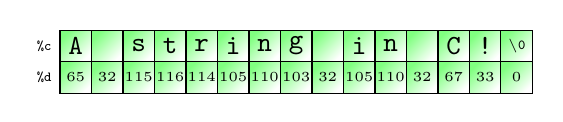
\begin{tikzpicture}[]
\foreach \x in {0.0, 0.4, ..., 5.6}
   \shadedraw [top color=green!50,shading angle=45] (\x,0) rectangle +(0.4,0.4);
\foreach \x in {0.0, 0.4, ..., 5.6}
   \shadedraw [top color=green!50,shading angle=45] (\x,0.4) rectangle +(0.4,0.4); \node at (0.2, 0.2) {\tiny65};
\node at (0.6, 0.2) {\tiny32};
\node at (1.0, 0.2) {\tiny115};
\node at (1.4, 0.2) {\tiny116};
\node at (1.8, 0.2) {\tiny114};
\node at (2.2, 0.2) {\tiny105};
\node at (2.6, 0.2) {\tiny110};
\node at (3.0, 0.2) {\tiny103};
\node at (3.4, 0.2) {\tiny32};
\node at (3.8, 0.2) {\tiny105};
\node at (4.2, 0.2) {\tiny110};
\node at (4.6, 0.2) {\tiny32};
\node at (5.0, 0.2) {\tiny67};
\node at (5.4, 0.2) {\tiny33};
\node at (5.8, 0.2) {\tiny0};

\node at (0.2, 0.6) {\tt A};
\node at (1.0, 0.6) {\tt s};
\node at (1.4, 0.6) {\tt t};
\node at (1.8, 0.6) {\tt r};
\node at (2.2, 0.6) {\tt i};
\node at (2.6, 0.6) {\tt n};
\node at (3.0, 0.6) {\tt g};
\node at (3.8, 0.6) {\tt i};
\node at (4.2, 0.6) {\tt n};
\node at (5.0, 0.6) {\tt C};
\node at (5.4, 0.6) {\tt !};
\node at (5.8, 0.6) {\tiny\tt $\backslash$0};

\node at (-0.2, 0.2) {\tiny\tt\%d};
\node at (-0.2, 0.6) {\tiny\tt\%c};
\end{tikzpicture}
\end{center}
\begin{itemize}
\item All strings in C are terminated by 0 (or {\tt \kt{'$\backslash$0'}}).
\item {\tt \kw{char}} values of 0-127 correspond to \emph{ASCII} codes, their use should be relatively consistent between different compilers.
\item All other values correspond to \emph{extended ASCII} codes, the representations of which vary considerably between compilers.
\end{itemize}
\end{frame}

\begin{frame}
\frametitle{Some useful {\tt char} Functions}
\begin{block}{For {\tt char}s}
\begin{tabular}{l p{200pt}}
\tt isalpha(c)&True (non-zero) if {\tt c} is from {\tt A-Z},{\tt a-z}\\
\tt isdigit(c)&True if {\tt c} if from {\tt 0-9}\\
\tt isalnum(c)&={\tt (isalpha(c) || isdigit(c))}\\
\tt islower(c)&True if {\tt c} is from {\tt a-z}\\
\tt isupper(c)&True if {\tt c} is from {\tt A-Z}\\
\tt d=tolower(c)&Convert to lowercase (if {\tt isupper(c)}), otherwise it returns {\tt c}\\
\tt d=toupper(c)&Convert to uppercase (if {\tt islower(c)}), otherwise it returns {\tt c}
\end{tabular}
\end{block}
\end{frame}

\begin{frame}
\frametitle{Some useful String Functions}
\begin{block}{\tt strlen(s)}
Returns the number of characters pointed to by {\tt s}, the trailing {\tt NULL} ({\tt \kt{'$\backslash$0'}}) is excluded!
\end{block}
\begin{block}{\tt strncpy(dest, source, length)}
Copies a maximum of {\tt length} characters from {\tt source} to {\tt dest}.
\end{block}
\begin{block}{\tt int strncmp(s1, s2, length)}
Compares a maximum of {\tt length} characters of {\tt s1} and {\tt s2}. Note that {\tt strncmp} returns 0 (usually false) for equality!
\end{block}
\end{frame}

\begin{frame}[fragile]
\frametitle{A String Demo}
\vspace{-0.2in}
\begin{semiverbatim}
\tiny
\kr\kl\kw{\#include} \kt{<stdio.h>}
\kl\kw{\#include} \kt{<string.h>}
\kl\kw{\#include} \kt{<stdlib.h>}
\kl\kw{\#include} \kt{<ctype.h>}
\kl
\kl\kw{int} main()
\kl\{
\kl   \kw{unsigned int} loop;
\kl   \kw{char} * string = \kt{"A string in C!"}, * copy;
\kl   printf(\kt{"strlen(string) = \%d\\n"}, strlen(string));
\kl   copy = (char *) calloc(strlen(string)+1, 1);
\kl   \kw{if} (!copy)
\kl   \{
\kl      fprintf(stderr, \kt{"Couldn't allocate buffer!\\n"});
\kl      \kw{return} -1;
\kl   \}
\kl   
\kl   strncpy(copy, string, strlen(string));
\kl   printf(\kt{"strncmp(string, copy) = \%d\\n"},
\kl         strncmp(string, copy, strlen(string)));
\kl         
\kl   \kw{for} (loop = 0; loop < strlen(copy); loop++)
\kl      copy[loop] = toupper(copy[loop]);
\kl      
\kl   printf(\kt{"modified copy = \\"\%s\\"\\n"}, copy);
\kl   printf(\kt{"strncmp(string, copy) = \%d\\n"},
\kl         strncmp(string, copy, strlen(string)));
\kl         
\kl   free(copy);
\kl   \kw{return} 0;
\kl\}
\end{semiverbatim}
\end{frame}

\begin{frame}[fragile]
\frametitle{Results from String Demo}
The program on the previous slide gives the following output:
\begin{semiverbatim}
strlen(string) = 14
strncmp(string, copy) = 0
modified copy = "A STRING IN C!"
strncmp(string, copy) = 32
\end{semiverbatim}
\begin{itemize}
\item Note that {\tt strncmp} returns {\tt 0} for \emph{equality} and non-zero otherwise.
\item Case insensitive string comparisons can be made using: {\tt strnicmp}.
\end{itemize}
\end{frame}


\begin{frame}[fragile]
\frametitle{Handling the command-line in C}
\begin{itemize}
\item So far, we have used the prototype: {\tt \kw{int} main(\kw{void})}.
\item UNIX and Windows support command-line arguments to programs, and these need to be passed to main somehow.
\item There is another prototype of {\tt main} we are allowed to use:\\
\begin{center}
\tt \kw{int} main(\kw{int} argc, \kw{char} ** argv)
\end{center}
\end{itemize}
The example below prints out the command-line arguments to a program:
\vspace{-0.1in}
\begin{semiverbatim}
\small
\kw{\#include} \kt{<stdio.h>}

\kw{int} main(\kw{int} argc, \kw{char} ** argv)
\{
   \kw{int} loop;
   \kw{for} (loop = 0; loop < argc; loop++)
      printf(\kt{"argv[\%d] = \%s\\n"}, loop, argv[loop]);
   \kw{return} 0;
\}
\end{semiverbatim}
\end{frame}


\newcommand{\scs}[1]{\scriptsize \sc#1}
\newcommand{\scc}[1]{$\mathtt{\backslash}$\tt#1}

\begin{frame}[fragile]
\frametitle{ASCII Table}
\resizebox{\textwidth}{!}{
\rowcolors[]{1}{blue!20}{blue!10}
\begin{tabular}{c| c c c c c c c c c c c c c c c c}
&0&1&2&3&4&5&6&7&8&9&A&B&C&D&E&F\\
\hline
0&\scc0&\scs soh & \scs stx & \scs etx&
\scs eot&\scs enq&\scs ack&\scc a&\scc b&\scc t&\scc n&
\scs vt&\scc f&\scc r&\scs so&\scs si\\
1&\scs dle&\scs dc1&\scs dc2&\scs dc3&\scs dc4
&\scs nak&\scs syn&\scs etb&\scs can&\scs em&\scs sub&
\scs esc&\scs fs&\scs gs&\scs rs&\scs us\\
2&\tt' '&\tt!&\tt"&\tt\#&\tt\$&\tt\%&\tt\&&\tt'&\tt(&\tt)&
\tt*&\tt+&\tt,&\tt-&\tt.&\tt/\\
3&\tt0&\tt1&\tt2&\tt3&\tt4&\tt5&\tt6&\tt7&\tt8&\tt9&\tt:&\tt;
&\tt<&\tt=&\tt>&\tt?\\
4&\tt@&\tt{A}&\tt{B}&\tt{C}&\tt{D}&\tt{E}&\tt{F}&\tt{G}&\tt{H}&
\tt{I}&\tt{J}&\tt{K}&\tt{L}&\tt{M}&\tt{N}&\tt{O}\\
5&\tt{P}&\tt{Q}&\tt{R}&\tt{S}&\tt{T}&\tt{U}&\tt{V}&\tt{W}&\tt{X}&
\tt{Y}&\tt{Z}&\tt[&$\mathtt{\backslash}$&\tt]&\tt\^&\tt\_\\
6&\tt`&\tt{a}&\tt{b}&\tt{c}&\tt{d}&\tt{e}&\tt{f}&\tt{g}&\tt{h}&
\tt{i}&\tt{j}&\tt{k}&\tt{l}&\tt{m}&\tt{n}&\tt{o}\\
7&\tt{p}&\tt{q}&\tt{r}&\tt{s}&\tt{t}&\tt{u}&\tt{v}&\tt{w}&
\tt{x}&\tt{y}&\tt{z}&\tt\{&\tt|&\tt\}&\tt\~&\scs del
\end{tabular}}
\begin{itemize}
\item Characters 0x00 to 0x1f (31) are \emph{non-printable}.
\item Characters 0x80 (128) to 0xff (255) are \emph{extended characters}.
\item We are going to have problems representing other languages using ASCII!
\end{itemize}
\end{frame}

\begin{frame}[fragile]
\frametitle{Internationalisation (i18n)}
There are two methods that C employs to overcome the limitations of {\tt \kw{char}}:
\begin{block}{Wide Characters \& Wide Strings (used in Windows)}
C has a wide character type called {\tt \kw{wchar\_t}}, a capital L is used to denote a wide character or wide string:
\vspace{-0.1in}
\begin{semiverbatim}
\kw{wchar_t} mwchar = L\kt{'a'};
\kw{wchar_t} * wideString = L\kt{"A wide string"};
\end{semiverbatim}
\end{block}

\begin{block}{Multibyte Characters (used in Linux)}
Another trick is to encode frequently used characters (such as numbers and Roman letters) using ASCII as normal, and for larger character sets (such as Hanzi) combine two or more {\tt \kw{char}}s together.
\end{block}
\end{frame}

\begin{frame}[fragile]
\frametitle{Unicode Sample}
\framesubtitle{A sample to convert from wide to multibyte, then print}
\vspace{-0.1in}
\begin{semiverbatim}
\tiny
\kr\kl\kw{\#include} \kt{<stdio.h>}
\kl\kw{\#include} \kt{<wchar.h>}
\kl\kw{\#include} \kt{<stdlib.h>}
\kl\kw{\#include} \kt{<locale.h>}
\kl
\kl\kw{int} main()
\kl\{
\kl   \kw{wchar_t} * unicodeString = L\kt{"a name:\\x8FEA\\x6587\\nMaths symbols:"}
\kl                             L\kt{"x\\x220A\\x2115\\x2204\\x222B\\x2202\\n"};
\kl   \kw{char} * mbString = NULL;
\kl   size_t mbSize;
\kl   \kc{/* select native locale */}
\kl   \kw{char} * locale = setlocale( LC_CTYPE, \kt{""});
\kl   printf(\kt{"MB_CUR_MAX = \%d\\n"}, MB_CUR_MAX);
\kl   printf(\kt{"sizeof(wchar_t) = \%d\\n"}, \kw{sizeof}(\kw{wchar_t}));
\kl   printf(\kt{"locale = \%s\\n"}, locale);
\kl
\kl   mbSize = (wcslen(unicodeString)+1)*MB_CUR_MAX;
\kl   mbString = (\kw{char} *) malloc(mbSize);
\kl   \kw{if} (!mbString)
\kl   \{
\kl      fprintf(stderr, \kt{"Unable to allocate multibyte buffer"});
\kl      \kw{return} -1;
\kl   \}
\kl
\kl   wcstombs(mbString, unicodeString, mbSize);
\kl   printf(\kt{"Multibyte: \%s\\n"}, mbString);
\kl   free(mbString); 
\kl   \kw{return} 0;
\kl\}
\end{semiverbatim}
\end{frame}

\begin{frame}
\frametitle{Multibyte Output}
\begin{itemize}
\item Logging in to a Linux box via PuTTY and using UTF-8 encoding, I get:
\begin{center}
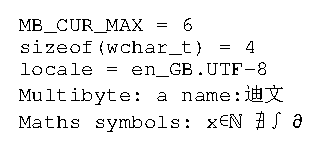
\includegraphics[width=0.5\textwidth]{unicodeoutput.eps}
\end{center}
\item This won't work properly for the Windows text console, as it doesn't allow for any unicode encodings. (If you set both the system and user locales to Chinese, then the Hanzi will display properly).
\end{itemize}
\end{frame}

\begin{frame}
\frametitle{C Keywords}
The following keywords are recognised by all C compilers as special commands. These words should not be used for variable names, function names etc.
\begin{center}
\begin{tabular}{l l l l}
\tt\kw{auto}&\tt\kw{break}&\tt\kw{case}&\tt\kw{char}\\
\tt\kw{const}&\tt\kw{continue}&\tt\kw{default}&\tt\kw{do}\\
\tt\kw{double}&\tt\kw{else}&\tt\kw{enum}&\tt\kw{extern}\\
\tt\kw{float}&\tt\kw{for}&\tt\kw{goto}&\tt\kw{if}\\
\tt\kw{int}&\tt\kw{long}&\tt\kw{register}&\tt\kw{return}\\
\tt\kw{short}&\tt\kw{signed}&\tt\kw{sizeof}&\tt\kw{static}\\
\tt\kw{struct}&\tt\kw{switch}&\tt\kw{typedef}&\tt\kw{union}\\
\tt\kw{unsigned}&\tt\kw{void}&\tt\kw{volatile}&\tt\kw{while}
\end{tabular}
\end{center}
\begin{itemize}
\item Exercise, look up the ones that have not been discussed in lectures.
\end{itemize}
\end{frame}

\begin{frame}
\frametitle{C Keywords - Discussion}
\begin{itemize}
\item {\tt\kw{auto}} is the complement of {\tt\kw{static}}, it is set by default thus seldom seen in code. \emph{DO NOT USE} - in the latest C++ standard, {\tt\kw{auto}} has a new meaning.
\item {\tt\kw{const}} specifies that a variable may not be changed once it's initialised. Can also be used in function prototypes to indicate read only arguments (i.e. read only arrays). Proper use of {\tt\kw{const}} is often referred to as \emph{const correctness}.
\item {\tt\kw{enum}} creates a unique type that assigns numerical values to symbolic names, e.g.\\
\begin{center}
\tt \kw{enum} suit \{clubs, diamonds, hearts, spades\};
\end{center}
\end{itemize}
\end{frame}

\begin{frame}
\frametitle{Preprocessor Keywords}
\begin{itemize}
\item We also have the following preprocessor keywords:
\begin{center}
\begin{tabular}{l l l}
\tt\kw{\#include}&\tt\kw{\#define}&\tt\kw{\#undef}\\
\tt\kw{\#if}&\tt\kw{\#ifdef}&\tt\kw{\#ifndef}\\
\tt\kw{\#elif}&\tt\kw{\#else}&\tt\kw{\#endif}\\
\tt\kw{\#error}&\tt\kw{\#line}&\tt\kw{\#pragma}
\end{tabular}
\end{center}
\vspace{0.2in}
\item The {\tt\kw{\#pragma}} directive is ``implementation specific''.
\end{itemize}
\end{frame}

\begin{frame}
\frametitle{Operator Precedence and Associativity}
\framesubtitle{From K\&R2:}
\begin{columns}
\begin{column}{9cm}
\resizebox{\textwidth}{!}{
\begin{tabular}{l| l}
Operators&Associativity\\
\hline
\tt () [] -> .&left to right\\
\tt ! $\sim$ ++ -- + - * \& (\emph{type}) \kw{sizeof}&right to left\\
\tt * / \%&left to right\\
\tt + -&left to right\\
\tt << >>&left to right\\
\tt < <= > >=&left to right\\
\tt == !=&left to right\\
\tt \&&left to right\\
\tt \^&left to right\\
\tt |&left to right\\
\tt \&\&&left to right\\
\tt ||&left to right\\
\tt ?:&right to left\\
\tt = += -= *= /= \%= \&= $\wedge$= |= <<= >>=&right to left\\
\tt ,&left to right
\end{tabular}}
\end{column}
\end{columns}
\end{frame}

\begin{frame}
\frametitle{Operator Precedence and Associativity - Examples}
\begin{exampleblock}{\tt a - b * c / d}
\begin{enumerate}
\item {\tt *} and {\tt /} are carried out before {\tt -} due to precedence.
\item {\tt *} is carried out before {\tt /} due to (left to right) associativity.
\end{enumerate}
\end{exampleblock}

\begin{alertblock}{\tt if (x \& MASK == 0)}
\begin{itemize}
\item {\tt ==} has a higher precedence than {\&} so is executed first!
\item To get what we originally intended, parentheses are needed:\\
\begin{center}
\tt \kw{if} ((x\& MASK) == 0)
\end{center}
\end{itemize}
\end{alertblock}

\begin{block}{If in doubt}
\begin{center}
Put brackets around things...
\end{center}
\end{block}
\end{frame}

{
\setbeamercolor{frametitle}{bg=red}
\begin{frame}[fragile]
\frametitle{More Pointers!}
\begin{itemize}
\item So far, we have seen examples of pointers to:
\begin{itemize}
\item native types (such as {\tt\kw{int}*}, {\tt\kw{float}*}, {\tt\kw{double}*}...),
\item something unknown ({\tt\kw{void}*}),
\item structures (such as {\tt FILE*}),
\item and pointers themselves (such as {\tt\kw{int}**}, {\tt\kw{double}**}...).
\end{itemize}
\item There is one more pointer type, a pointer to a \emph{function}.
\end{itemize}

\begin{block}{Why point to functions?}
C code is often re-used between projects. Mathematical routines such as ones to find roots of functions, become extremely limited if they are tied down to a specific case.
\end{block}

\begin{exampleblock}{Declaring a pointer to a function}
One way is to use a {\tt\kw{typedef}}:
\vspace{-0.1in}
\begin{center}
\tt \kw{typedef} \kw{double} (* fx)(\kw{double} x);
\end{center}
\end{exampleblock}
\end{frame}
}

\begin{frame}[fragile]
\frametitle{Function Pointers - An example}
\vspace{-0.2in}
\begin{semiverbatim}
\tiny
\kw{\#include} \kt{<stdio.h>}
\kw{typedef double} (* fx)(\kw{double} x);

\kw{double} newtonSolve(fx func, fx grad, \kw{double} guess)
\{
   \kw{unsigned int} loop;
   \kw{for} (loop = 0; loop < 10; loop++) guess -=func(guess)/grad(guess);
   \kw{return} guess;
\}

\kw{double} sample(\kw{double} x)
\{
   \kw{return} x*x-2.0;
\}

\kw{double} dsample(\kw{double} x)
\{
   \kw{return} 2.0*x;
\}

\kw{int} main()
\{
   \kw{double} sol = newtonSolve(sample, dsample, 1.0);
   printf(\kt{"Solution = \%.15lg\\n"}, sol);     
   printf(\kt{"Residue = \%lg\\n"}, sample(sol));
   \kw{return} 0;
\}
\end{semiverbatim}
This should get you started with exercise \# 5.
\end{frame}

\begin{frame}
\frametitle{Don't Do it All Yourself!}
\begin{itemize}
\item As you have seen from the exercises, writing functions to solve equations such as cubics can become complicated (especially when rounding error needs to be minimised).
\item A lot of people have spent a considerable amount of time attempting to perfect implementations of mathematical functions.
\item Routines written by a third party are packaged in \emph{libraries}.
\end{itemize}
\end{frame}

\begin{frame}
\frametitle{Using Fortran Code}
\begin{itemize}
\item Good news! Scientific programming has been going on for over 60 years (counting from Colossus) in Britain.
\item Unfortunately a lot of this has been carried out in Fortran.
\end{itemize}
\begin{block}{\tt f2c}
Bell Labs have released a program called {\tt f2c} which converts Fortran source code to C. The output from {\tt f2c} is usually not very human friendly, but it does at least compile.
\end{block}
\end{frame}

\begin{frame}
\frametitle{GNU Scientific Library - GSL}
GNU have released their C Scientific Library:
\begin{center}
\url{http://www.gnu.org/software/gsl/}
\end{center}

\begin{itemize}
\item It is managed by scientists at Los Alamos, and is very comprehensively documented.
\item GSL requires gcc (for Windows users, Cygwin can be used).
\end{itemize}

\begin{alertblock}{Licensing}
``GSL can be used internally ("in-house") without restriction, but only redistributed in other software that is under the GNU GPL.''
\end{alertblock}
\end{frame}

\begin{frame}[fragile]
\frametitle{GSL Example}
\vspace{-0.2in}
\begin{semiverbatim}
\small
\kw{\#include} \kt{<stdio.h>}
\kw{\#include} \kt{<gsl/gsl_sf_bessel.h>}

\kw{int} main()
\{
   \kw{double} x = 0.0;

   printf(\kt{"Enter x \\n"});
   scanf(\kt{"\%lf"}, &x);
   printf(\kt{"J0(\%g) = \%.18e\\n"}, x, gsl_sf_bessel_J0(x));

   return 0;
\}
\end{semiverbatim}
Compile this using the command-line:
\begin{alertblock}
\tt gcc gsl-sample.c -lgsl  -lgslcblas -lm -o gsl-sample
\end{alertblock}
\end{frame}

\begin{frame}
\frametitle{NAGLIB}
The Numerical Algorithms Group, based in Oxford, maintain a software library called NAGLIB.
\begin{itemize}
\item Imperial College have signed a site license for NAGLIB.
\item It can be installed on departmental machines upon request.
\item You are allowed to install it on your home machines.
\end{itemize}
\end{frame}

\begin{frame}
\frametitle{General Numerical Software}
\begin{center}

\includegraphics[width=0.2\textwidth]{netlib.eps}
\end{center}
The Netlib Repository contains a lot of very useful numerical codes and papers. It is definitely worth having a route through their website:
\begin{center}
\url{www.netlib.org}
\end{center}
\end{frame}

\begin{frame}
\frametitle{JPEG Manipulation}
\begin{itemize}
\item The Independent JPEG Group, release a freeware JPEG (compressor/decompressor) library.
\item Code is available from \url{http://www.ijg.org}; the most recent version as of writing is 8a (dated 28-Feb-2010).
\item To use the code in Visual Studio one needs to rename some project files (please refer to {\tt install.txt} for details).
\item Example code is included that demonstrates the proper use of the library, for an example of decompression please refer to {\tt djpeg.c}.
\end{itemize}


\end{frame}

\begin{frame}
\frametitle{Graphics Programming in C}
\begin{alertblock}{Avoid it if you can!}
Most of the time scientific output can be plotted quite well by GNUplot, Maple and Matlab.
\end{alertblock}
\begin{block}{If you still want to...}
\begin{columns}
\begin{column}{1.5cm}
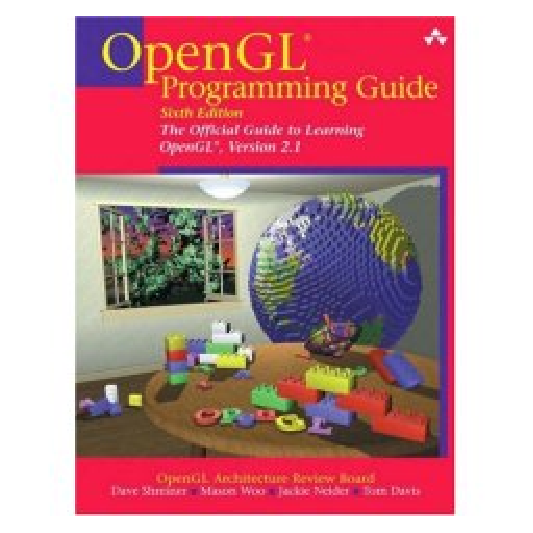
\includegraphics[width=1.6\textwidth]{opengl}
\end{column}
\begin{column}{8cm}
I recommend that you program in OpenGL as it is portable across architectures and makes use of the graphics hardware in machines. I learnt OpenGL from the ``Red Book''; OpenGL Programming Guide: The Official Guide to Learning OpenGL.
\end{column}
\end{columns}
\end{block}
\begin{exampleblock}{Example Code}
I have placed an OpenGL sample on my website, it also conveniently demonstrates almost all the C we have covered in this course!
\end{exampleblock}
\end{frame}

\begin{frame}[fragile]
\frametitle{Calling Fortran from C - the C {\tt main} function}
\begin{semiverbatim}
\small
\kw{\#include} \kt{<stdio.h>}

\kw{extern double} ffunc01_(\kw{double} *x);

\kw{double} callfortran(\kw{double} x)
\{
   \kw{return} ffunc01_(&x);
\}

\kw{int} main()
\{
   \kw{double} x = 1.0;
   
   printf(\kt{"Hello from C!\\n"});
   printf(\kt{"fsub(%g) = %g\\n"}, x, callfortran(x));
   \kw{return} 0;
\}
\end{semiverbatim}
\end{frame}

\begin{frame}[fragile]
\frametitle{Calling Fortran from C - The Fortran Function}
\begin{semiverbatim}
\small
\kw{function} ffunc01(x)
   \kw{real}(\kw{kind}=8), \kw{intent}(\kw{in}) :: x
   \kw{real}(\kw{kind}=8)             :: ffunc01
   
   ffunc01 = 10*x + 1   
   print *, \kt{'In fortran, received x = '}, x
   print *, \kt{'returning'}, ffunc01   
\kw{end function}
\end{semiverbatim}
\begin{itemize}
\item We explicitly specify {\tt kind=8}, i.e. {\tt double} precision.
\item In {\tt g95}, all exported functions have a trailing underscore.
\item Fortran arguments to functions are pointers.
\end{itemize}
\end{frame}

\begin{frame}[fragile]
\frametitle{Calling C from Fortran - Fortran Interface}
\begin{semiverbatim}
\scriptsize
\kw{module} cmodule
   \kw{implicit none}
\kw{contains}

   \kw{function} my_func(x)
      \kw{real}, \kw{intent}(\kw{in}) :: x
      \kw{real}             :: my_func
      \kw{real}(\kw{kind}=8)     :: tmp
            
      \kw{interface}
         \kw{function} cfunc01(x)
            \kw{real}(\kw{kind}=8), \kw{intent}(\kw{in}) :: x
            \kw{real}(\kw{kind}=8)             :: cfunc01
         \kw{end function} cfunc01
      \kw{end interface}
      
      tmp = x
                  
      my_func = cfunc01(tmp)
   \kw{end function} my_func
\kw{end module} cmodule
\end{semiverbatim}
\end{frame}

\begin{frame}[fragile]
\frametitle{Calling C from Fortran - Fortran entry point}
\begin{semiverbatim}
\small
\kw{program} test
   \kw{use} cmodule
   \kw{implicit none}
   
   \kw{real} :: myx = 26.0980
   
   print *, \kt{'myx = '}, myx
   print *, \kt{'my_funx(myx) = '}, my_func(myx)
\kw{end program}
\end{semiverbatim}
\begin{itemize}
\item We must compile the {\tt cmodule} \emph{before} the entry point.
\item This is due to Fortran .mod files (think auto-generated .h files).
\end{itemize}
\end{frame}

\begin{frame}[fragile]
\frametitle{Calling C from Fortran - The C function}
\begin{semiverbatim}
\scriptsize
\kw{\#include} \kt{<stdio.h>}

\kw{double} cfunc01_(\kw{double} * x)
\{
   \kw{double} retval = (*x)*(*x) - 1.0;
   printf(\kt{"In cfunc01(): received x = %g, returning: %g\\n"},
          *x, retval);
   \kw{return} retval;
\}
\end{semiverbatim}
\begin{itemize}
\item The arguments to the c function are pointers.
\item {\tt cfunc01} is referenced from the {\tt cmodule} interface.
\item We add a trailing underscore to the function name.
\item Function name translation in object files is known as \emph{name mangling}.
\end{itemize}
\begin{alertblock}{}
\begin{center}
Different compilers have different calling conventions!
\end{center}
\end{alertblock}
\end{frame}

\begin{frame}[fragile]
\frametitle{Linking Fortran and C - Putting it all together}
\begin{exampleblock}{}
\begin{semiverbatim}
\scriptsize
.SUFFIXES: .f90
CFLAGS = -pedantic -ggdb -Wall -ansi
FFLAGS = -ggdb
LFLAGS = -lm
CC = gcc
F90 = g95
CLEANFILES = fmain.o csub.o demo1 fmod.o cmodule.mod demo1.exe \\
             cmain.o demo2 demo2.exe ffunc.o

all:    demo1 demo2

demo1:  cmain.o ffunc.o
        $(F90) cmain.o ffunc.o -o demo1

demo2:  fmod.o fmain.o csub.o
        $(F90) fmod.o fmain.o csub.o -o demo2
 
clean:
        touch $(CLEANFILES)
        rm $(CLEANFILES)

.f90.o:
        $(F90) $(FFLAGS) -c $*.f90
\end{semiverbatim}
\end{exampleblock}
\end{frame}

\begin{frame}[fragile]
\frametitle{Running the codes}
Running the first demo:
\begin{semiverbatim}
\small
$ ./demo1 
Hello from C!
 In fortran, received x =  1.  returning 11.
fsub(1) = 11
\end{semiverbatim}

and the second demo:
\begin{semiverbatim}
\small
$ ./demo2 
 myx =  26.098
In cfunc01(): received x = 26.098, returning: 680.106
 my_funx(myx) =  680.1056
\end{semiverbatim}
\end{frame}

\begin{frame}
\frametitle{Moving on to C++}
\begin{block}{What is it?}
\begin{itemize}
\item C++ can be thought of very loosely as an object oriented extension to C.
\item The C++ standard is over twice as big as the C standard.
\item C++ is in the process of changing (at the time of writing C++0x is being adopted by compilers).
\end{itemize}
\end{block}
\begin{exampleblock}{References}
\begin{columns}
\begin{column}{1cm}

\includegraphics[width=2.6\textwidth]{deitelnew.eps}
\end{column}
\begin{column}{8cm}
\begin{itemize}
\item One good book that has been brought to my attention is ``C++ How to Program 7th Edition'' by Harvey and Paul Deitel published in 2010.
\item Before buying any C++ book, make sure that it is recent, and that you like the writing style.
\end{itemize}
\end{column}
\end{columns}
\end{exampleblock}
\end{frame}

\begin{frame}
\frametitle{Moving on to C\# or Java?}
Java and C\# belong to a different class of language.
\begin{columns}
\begin{column}{0.55\textwidth}
\begin{itemize}
\item Java and C\#, both target \emph{virtual machines}.
\item Pointers are hidden from the user in C\# and completely absent from Java.
\item Most memory allocation and de-allocation is done automatically, via
\emph{garbage collection}.
\item Java code can target multiple platforms,
C\# is supported only on Microsoft platforms.
\end{itemize}
\end{column}
\begin{column}{0.7\textwidth}
\hspace{-0.57in}\rlap{\includegraphics[width=10.0cm]{comparison}}
\end{column}
\end{columns}
\end{frame}

\begin{frame}
\frametitle{C\# References}
\begin{block}{Book}
\begin{columns}
\begin{column}{1cm}

\includegraphics[width=2.0\textwidth]{csharp.eps}
\end{column}
\begin{column}{0.8\textwidth}
\begin{itemize}
\item ``Pro C\# 2008 and the .NET 3.5 Platform, Fourth Edition'' by Andrew Troelsen,
appears to be up-to-date and comprehensive.
\item I would recommend you skim through a copy before buying. (.Net 4.0 is out now).
\end{itemize}
\end{column}
\end{columns}
\end{block}
\begin{exampleblock}{MSDN}
The definitive (and free) source of information for Microsoft Platforms is the MSDN, the C\# documentation is browseable at:\\
{\footnotesize \url{http://msdn.microsoft.com/en-gb/library/kx37x362.aspx}}
\end{exampleblock}

\end{frame}

\end{document}
